%OnDieDecap_Model.tex
%
\section{Supply Modelling Basics for High-Speed IC Design}
%------------------------------------------------------------------------------
\par The purpose of this text is to provide a basic representation of power supply
networks in a way that is useful for circuit design.  With the intuition obtained
from this representation, the reader should be able to make informed decisions
with respect to the decoupling strategy. These concepts can be applied at all
stages of the design, starting with individual circuit blocks on the IC itself,
adjacent on-die power grids, package-level supply networks, and also board-level
traces, planes, capactiors, etc. leading all the way to back to the regulators.
%
\subsection{First-Order On-Die Supply Network Model}
%------------------------------------------------------------------------------
\par To avoid paralysis from an overwhelmingly large number of possible supply
network configurations, it is best to start with a simple first-order model
(Fig.~\ref{fig:Decap_1storder_LVDDLVSS}):
%
\begin{itemize}[noitemsep]
%\begin{enumerate}[\itemsep=0em]
\item Ideal short between all $VDDx$/$VSS$ package pins on the PCB side.
\item Ideal short between all $VDDx$/$VSS$ pins on the die side.
\item Ideal voltage supply feeding $VDDx$/$VSS$ package pins on the PCB side.
\item Purely inductive package characteristics between the pins located on the PCB interface, and those on the wafer (die) pads.
\end{itemize}
%
\begin{figure}[!ht]
	\centering
	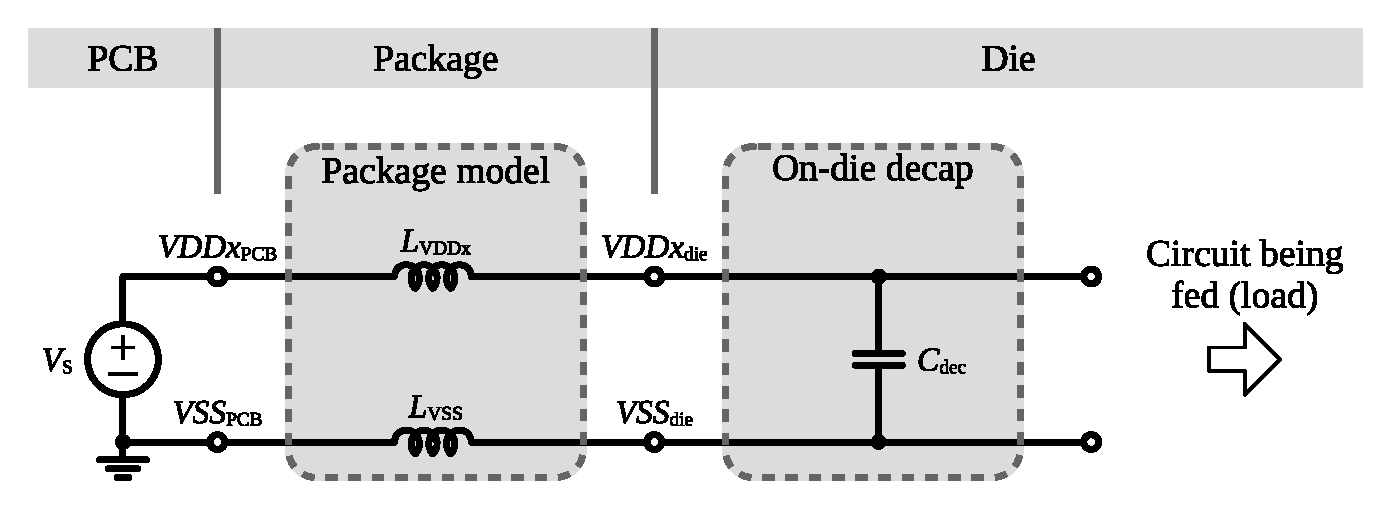
\includegraphics[scale=0.6]{Decap_1storder_LVDDLVSS}
	\caption{First-order supply model with on-die decoupling.}
\label{fig:Decap_1storder_LVDDLVSS}%############################################
\end{figure}
%
\par Note that we can lump together $L_\mathrm{pkg}=L_\mathrm{VDD}+L_\mathrm{VSS}$
while still maintaining the correct $I$--$V$ relationships between
$VDDx_\mathrm{die}$ \& $VSS_\mathrm{die}$ (Fig.~\ref{fig:Decap_1storder}).
In fact, the 2-port network representation of the package model remains
unchanged by this transformation.
%
\begin{figure}[!ht]
	\centering
	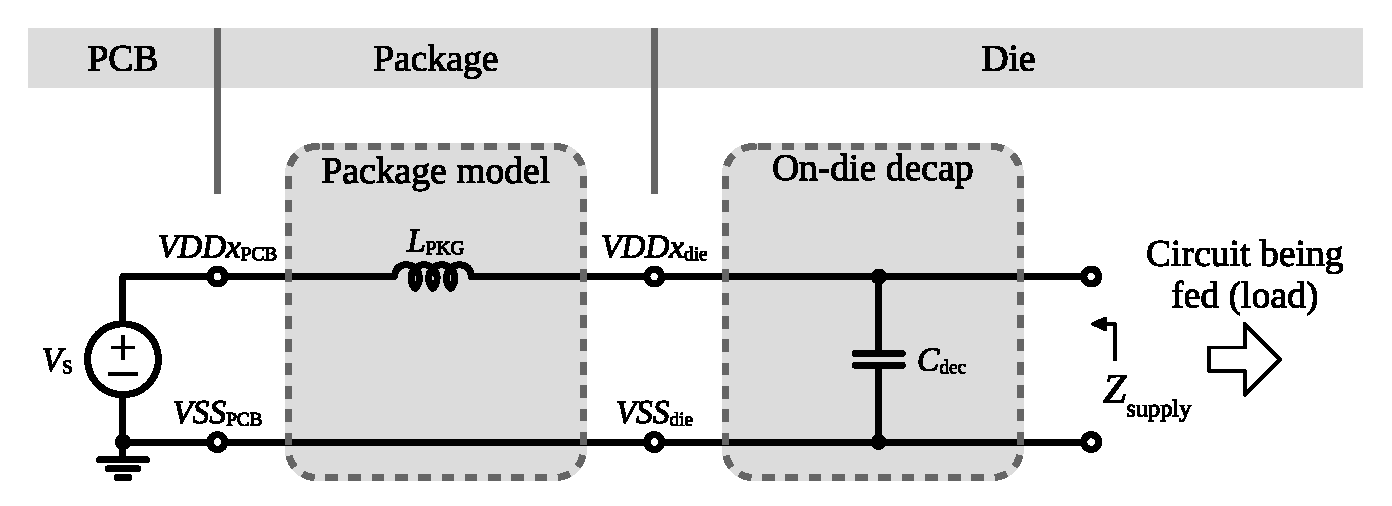
\includegraphics[scale=0.6]{Decap_1storder_LPKG}
	\caption{\emph{Simplified} first-order supply model ($L_\mathrm{pkg}$) with on-die decoupling.}
\label{fig:Decap_1storder}%#####################################################
\end{figure}
%
\par The principal advantage of this $L_\mathrm{pkg}$ reduction is that
simulators typically have less difficulty computing complex circuit responses
when circuits are connected directly to node 0 (ground). It also visually
simplifies the supply model a bit. Admittedly, applying such a simplification to
a \emph{4-port representation} of the package would hide certain non-critical
supply behaviours (most notably $VDD_\mathrm{die}$--$VSS_\mathrm{die}$
common-mode bounce).  In other words, the main drawback to using a single
effective $L_\mathrm{pkg}$ is to lose sight of the $VSS_\mathrm{die}$ supply
bounce relative to $VSS_\mathrm{PCB}$ (which people often imagine represents
the "real" ground).
%
\subsection{Supply Output Impedance, $Z_\mathrm{supply}$}
%------------------------------------------------------------------------------
\par A good way to visualize supply network characteristics is through the
supply impedance observed looking in from its connection to the load circuit.
Ideally, the supply should exhibit little voltage variation when the load
circuit draws current. This is the reason designers are interested in the
$I{\Rightarrow}V$ (or impedance) relationship at the load.
%
\par\noindent By selecting reasonable parameters for the model in
Fig.~\ref{fig:Decap_1storder}, the supply impedance profile in
Fig.~\ref{fig:Zsupply_1storder_nodamp} is obtained:
%
\begin{itemize}[noitemsep]
\item $L_\mathrm{pkg}=250\pH$.
\item $C_\mathrm{dec}=10\nF$.
\end{itemize}
%
\begin{figure}[!ht]
	\centering
	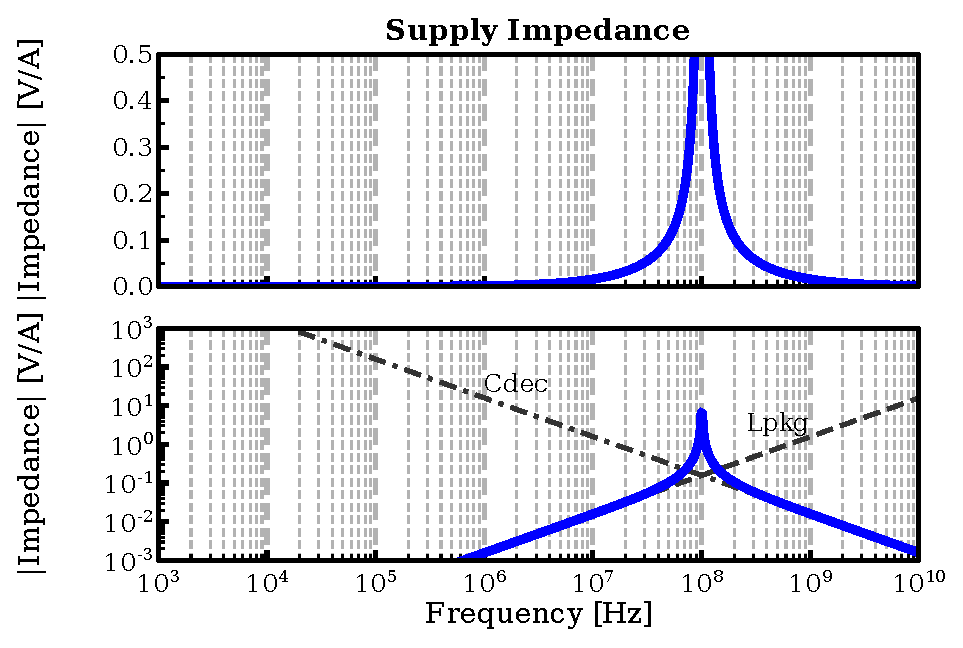
\includegraphics[scale=0.6]{Zsupply_1storder_nodamp}
	\caption{Supply impedance of first order model in Fig.~\ref{fig:Decap_1storder}.}
\label{fig:Zsupply_1storder_nodamp}%############################################
\end{figure}
%
\par Those familiar with supply decoupling solutions will notice
Fig.~\ref{fig:Zsupply_1storder_nodamp} exhibits significant resonance at
$100\MHz$. This effect is undesireable.
%
\subsection{Adressing the High-$Q$ Resonance}
%------------------------------------------------------------------------------
\par To reduce the resonant effect observed in Fig.~\ref{fig:Zsupply_1storder_nodamp},
one must de-$Q$ the supply at $100\MHz$.  A simple way to achieve this is
to add a shunt resistor, $R_\mathrm{damp}$, in parallel with $C_\mathrm{dec}$.
Unfortunately, this solution would draw an unacceptable amount of power from
the supplies. To circumvent this issue, a large DC-blocking capacitor,
$C_\mathrm{damp}$, is added in series with the damping resistor, as
illustrated in Fig.~\ref{fig:Decap_1storder_damp}.
%
\begin{figure}[!ht]
	\centering
	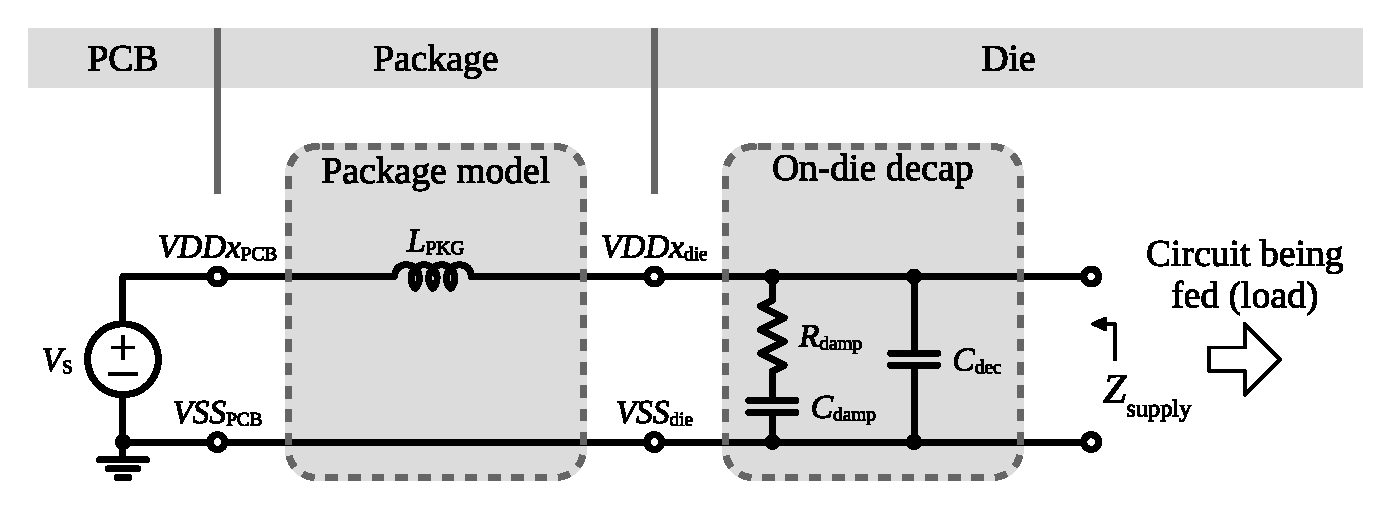
\includegraphics[scale=0.6]{Decap_1storder_Cdamp}
	\caption{First-order supply model with \emph{damped} on-die decoupling ($C_\mathrm{damp}$).}
\label{fig:Decap_1storder_damp}%###############################################
\end{figure}
%
\par A practical design point for this damped solution is to target a value of
$Q=1$. If we ignore the DC-blocking $C_\mathrm{damp}$, it is straightforward
to find a reasonable value for $R_\mathrm{damp}$ given that:
%
\begin{equation}
	Q \defAs \left |\frac{\imag{Y}}{\real{Y}}\right |
\end{equation}
%
\par\noindent Substituting in our parallel decoupling impedance, 
$Y=1/R_\mathrm{damp} + j\omega C_\mathrm{dec}$, we get:
\begin{equation}
	Q_\mathrm{damp} = \frac{\omega_\mathrm{res} C_\mathrm{dec}}{1/R_\mathrm{damp}}
\end{equation}
%
\par\noindent The target value for our damping resistor is therefore
obtained directly by letting $Q=1$:
\begin{equation}
	R_\mathrm{damp} = \frac{1}{2\pi f_\mathrm{res}C_\mathrm{dec}}
\end{equation}
%
\par Finally, to ensure the $R_\mathrm{damp}$--$C_\mathrm{damp}$ branch is
dominated by $R_\mathrm{damp}$ @ $f_\mathrm{res}$, we simply need to select a
value of $C_\mathrm{damp} \gg C_\mathrm{dec}$ (a factor of 5 seems reasonable).
Thus, we obtain the following new component parameters for our decoupling
solution:
\begin{itemize}[noitemsep]
\item $R_\mathrm{damp}=0.159\Ohm$.
\item $C_\mathrm{damp}=5 C_\mathrm{dec}=50\nF$.
\end{itemize}
%
\par\noindent The impedance profile for this newly damped supply response is
given in Fig.~\ref{fig:Zsupply_1storder}.
\begin{figure}[!ht]
	\centering
	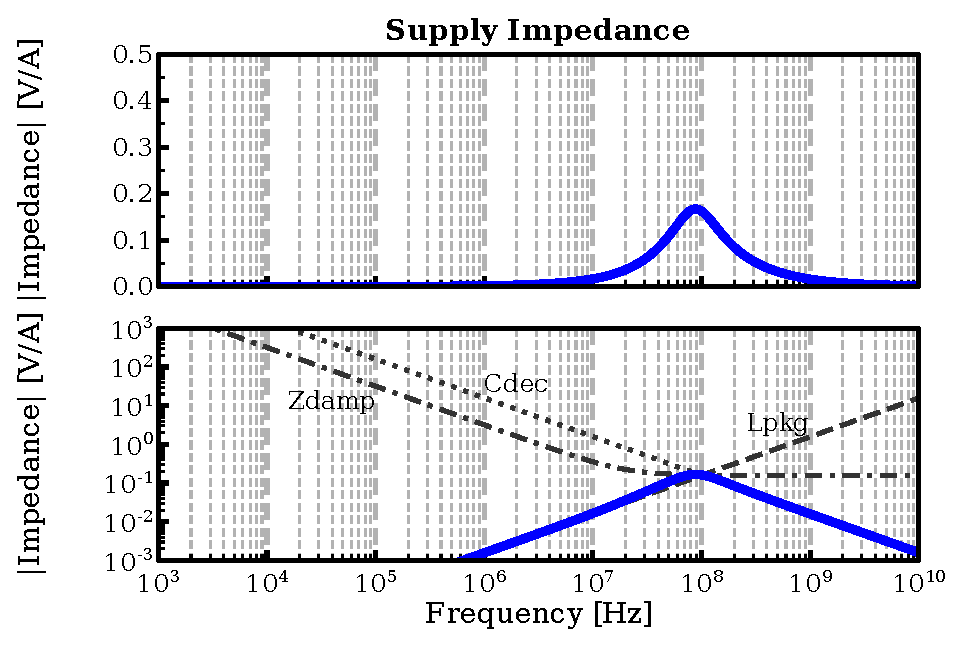
\includegraphics[scale=0.6]{Zsupply_1storder}
	\caption{Supply impedance of the (damped) first order model in Fig.~\ref{fig:Decap_1storder_damp}.}
\label{fig:Zsupply_1storder}%##################################################
\end{figure}
%
\section{Discrpancies in First-Order Capacitor Model}
%------------------------------------------------------------------------------
\par Experienced supply designers might be wary of a certain feature missing from the
impedance profile in Fig.~\ref{fig:Zsupply_1storder}: Typical impedance
profiles for discrete decoupling capacitors tend to rise with increasing $f$.
This is due to the physical length of the capacitor, resulting in a
corresponding parasitic (effective) series inductance ($ESL$).  The first-order
$RLC$ model in Fig.~\ref{fig:Decap_DiscreteModel} captures this effect
with $L_\mathrm{ESL}$. The net impedance profile for this first-order model
exhibits the characteristic "V" shape observed in discrete capacitors.
%
\begin{figure}[!ht]
	\centering
	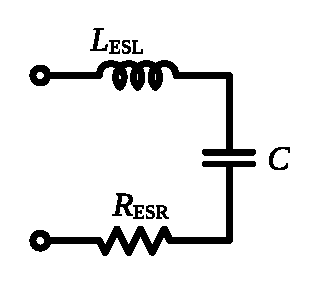
\includegraphics[scale=0.6]{Decap_DiscreteModel}
	\caption{First order model of a discrete decoupling capacitor component.}
\label{fig:Decap_DiscreteModel}%################################################
\end{figure}
%
\par To compensate for parasitic $L_\mathrm{ESL}$, supply networks typically
resort to adding multiple discrete bypass (decoupling) capacitors for each chip
on the PCB. Bypass capacitors with staggered frequency responses tend to be
selected in a way that maintains a low impedance profile at the chip pins
(Fig.~\ref{fig:Zsupply_PCB}).
%
\begin{figure}[!ht]
	\centering
	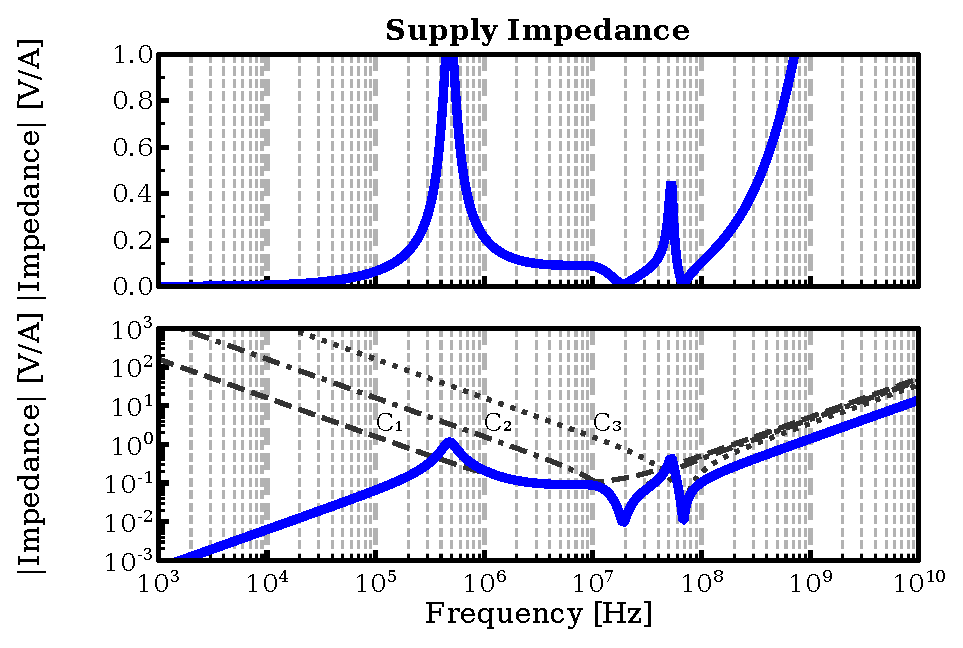
\includegraphics[scale=0.6]{Zsupply_PCB}
	\caption{PCB-level supply impedance profile (incl. discrete decoupling capacitors).}
\label{fig:Zsupply_PCB}%###################################################
\end{figure}
%
\par Ideally, on-chip capacitors should be located \emph{very} close to the
load circuit to ensure negligible values of $L_\mathrm{ESL}$. It
therefore follows that our models for on-die decoupling capacitors need not
exhibit the characteristic "V" impedance profile (at least not to a
first-order).
%
\section{An Intuition for Supply Transients}
%------------------------------------------------------------------------------
\par A good way to build up an intuition for supply transients is to experiment
with realistic transient current profiles generated by actual circuits. You don't
need fancy 2.5D/3D models of the power supply networks to get userful results.
Even the simple first-order model from Fig.~\ref{fig:Decap_1storder_damp} can be
very insightful.  Note that, to minimize the complexity of your simulation, it
is often sufficient to supply the circuits with an ideal voltage source. The
resulting current profiles should remain representative of the actual draw on
the supply newtwork. A rough schematic for such a simulation testbench is
provided in Fig.~\ref{fig:Testbench_SupplyTransient}.
%
\begin{figure}[!ht]
	\centering
	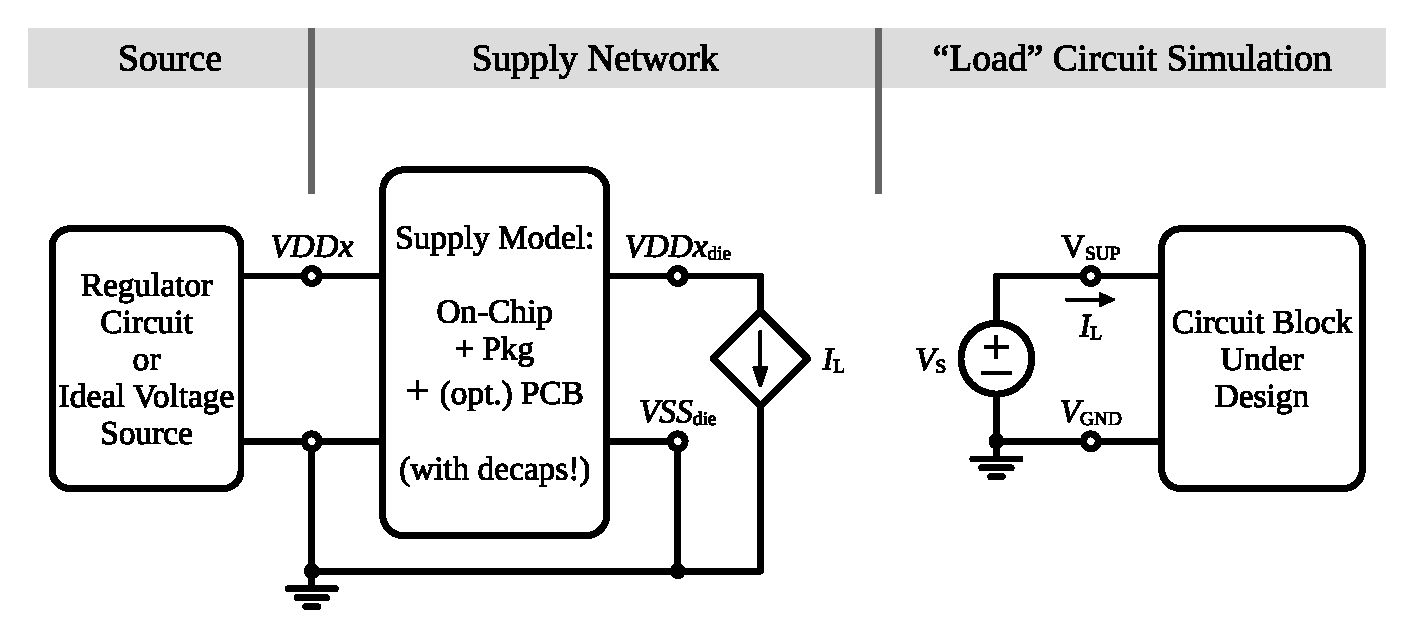
\includegraphics[scale=0.6]{Decap_CodesignTestbench}
	\caption{Testbench for supply transients using realistic current profiles.}
\label{fig:Testbench_SupplyTransient}%##########################################
\end{figure}
%
\par For reference, Fig.~\ref{fig:Supplybounce} includes simulation results for
a trivial circuit toggling a $400\fF$ load through $50\Ohm$ pull-up/down
resistors. Note that the $VDD$--$VSS$ supply exhibits quite a bit of
peak-to-peak bounce since it is relies on a little on-die decoupling
($C_\mathrm{dec}=1\pF$). In fact, a small value of $C_\mathrm{dec}$ was
specifically chosen to ensure the resultant supply bounce was clearly visible.
%
\begin{figure}[!ht]
	\centering
	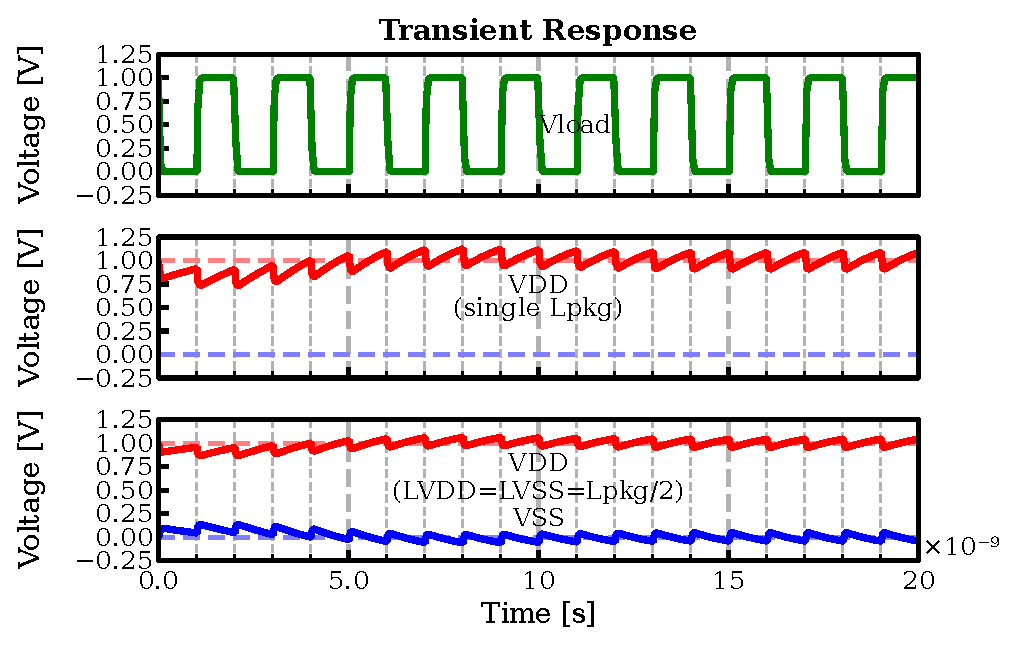
\includegraphics[scale=0.6]{supplybounce}
	\caption{Supply transients for $1\ns$--periodic toggle of a $400\pF$ load through $50\Ohm$ pull-up/down resistors.}
\label{fig:Supplybounce}%#######################################################
\end{figure}
%
\par For completeness, the supply response generated by leaving modelled
package inductances in their respective $VDD$ \& $VSS$ paths is included in the
bottom-most graph of Fig.~\ref{fig:Supplybounce} (assumes
$L_\mathrm{VDD}=L_\mathrm{VSS}=L_\mathrm{pkg}/2$). As might be expected, this
model shows how supply bounce is actually shared between the two supply nets,
while nonetheless exhibiting the same differential $VDD-VSS$ signature
computed for the combined--$L_\mathrm{pkg}$ simplification.
%
\section{Co-design Strategy: A 3-Step Process}
%------------------------------------------------------------------------------
\par It is normally bad practice to wait until top-level chip assembly to
start adding components like decoupling capacitors. When tapeout approaches,
designers are already busy scrambling to tie up other loose ends.
Having an effective means of integrating a decoupling solution during
the design stage of individual circuit blocks would be much more
productive.
%
\subsection{Critical assumption: $f_\mathrm{res}$ is known}
%------------------------------------------------------------------------------
\par Typically, little is known about the power supply network during the
block-level design stage.  A reasonable starting point is therefore to assume the
value of $f_\mathrm{res}$ is known. Since many practical designs appear to
exhibit a $100-250\MHz$ resonance between the on-die decoupling capacitance
\& the series supply inductance ($f_\mathrm{res}$), it seems reasonable
to start designing for something like:
\begin{equation}
	f_\mathrm{res}=100\MHz
\end{equation}
%
\par With a reasonable value of $f_\mathrm{res}$ in hand, designers can
assign a certain amount of decoupling to each individual circuit block
($C_\mathrm{dec}^\mathrm{blk}$), then compute the package inductance
"allocated" to those same blocks ($L_\mathrm{pkg}^\mathrm{blk}$).
Similarly, a shunt damping resistor ($R_\mathrm{damp}^\mathrm{blk}$)
can be computed, along with its DC-blocking capacitance. The relevant
model equations are provided below for reference:
%
\begin{equation}
	L_\mathrm{pkg}^\mathrm{blk} = \frac{1}{(2\pi f_\mathrm{res})^2 C_\mathrm{dec}^\mathrm{blk}}
\end{equation}
\begin{equation}
	R_\mathrm{damp}^\mathrm{blk} = \frac{1}{2\pi f_\mathrm{res}C_\mathrm{dec}^\mathrm{blk}}
\end{equation}
\begin{equation}
	C_\mathrm{damp}^\mathrm{blk} = 5C_\mathrm{dec}^\mathrm{blk}
\end{equation}
%
\subsection{The 3-Step Decoupling Strategy}
%------------------------------------------------------------------------------
\par The co-design strategy proposed in this text requires adding decoupling
capacitors during the block-level simulation \& layout steps. Specifically, the
following 3 steps should be applied for each designed block:
%
\begin{enumerate}[noitemsep]
\item Pick an arbitrary initial value of $C_\mathrm{dec}^\mathrm{blk}=1\pF$, and co-simulate the supply signature corresponding to the operation of said circuit (Apply testbench described in Fig.~\ref{fig:Testbench_SupplyTransient} with first-order package model from Fig.~\ref{fig:Decap_1storder_damp}).
\item Determine the scaling factor, $k$, that reduces supply bounce to within acceptable limits.
\item Add high-$Q$ decoupling capacitors to meet this $C_\mathrm{dec}^\mathrm{blk}=k\times 1\pF$ requirement \emph{inside} the block-level layout (do not wait for top-level assembly).
\end{enumerate}
%
\subsection{Placement of On-Die Decoupling Capacitors}
%------------------------------------------------------------------------------
\par To ensure optimum effectiveness of the high-$Q$ decoupling capacitors
supplying higher-frequency transient currents, all devices associated with
$C_\mathrm{dec}^\mathrm{blk}$ should be located right next to the supplied
blocks. Associated supply metalization should also be generous and short in
order to minimize both series inductance and resistance.
%
\par On the other hand, damping capacitors $C_\mathrm{damp}$ (and assoicated
$R_\mathrm{damp}$) can be located further away, provided the distance does
not result in excessive levels of parasitic inductance ($ESL$). In other words,
parasitic series inductance must not degrade the ability of damping
resistors/capacitors to de-$Q$ the package--$C_\mathrm{dec}$ resonator.
%
\section{Designing Outwards: IC$\Rightarrow$PCB$\Rightarrow$Regulator}
%------------------------------------------------------------------------------
\par To generate more accurate representations of impedance profiles and
supply transients, the basic process outlined in this text can be
repeated with the following refinements:
%
\begin{itemize}[noitemsep]
\item 1st order PCB supply model + decoupling devices.
\item 2.5D/3D package parasitics (+ decoupling, if present).
\item 2.5D/3D PCB supply model + decoupling devices.
\item Schematic model of the regulator block.
\end{itemize}
%
\section{Supplemental Reading Material}
%------------------------------------------------------------------------------
\par\noindent Suggested reading:
\par%
\cite{tr:Carter_2001}\cite{tr:Martin_Dateunkn}
\cite{tr:ADI_2009}\cite{tr:Zumbahlen_2012}\cite{tr:Kester_2017}
\cite{tr:Renesas_2011}
%
%Last line
